%%%%%%%%%%%%%%%%%%%%%%%%%%%%%%%%%%%%%%%%%%%%%%%%%%%%%%%%%%%%
% % Title and the authors % %
%%%%%%%%%%%%%%%%%%%%%%%%%%%%%%%%%%%%%%%%%%%%%%%%%%%%%%%%%%%%
\title{Lagrange Multipliers}
\author{ Gabriela Georgieva \\ Angelina Kuznetsova \\ Fedor Shafranov} \date{\today } 
\documentclass[]{article}

\usepackage{graphicx}
\usepackage[utf8]{inputenc}
\usepackage{setspace}
\usepackage{amsthm}
\usepackage{amssymb}
\usepackage{amsmath}
\usepackage{hyperref}
\usepackage{tikz}
\usepackage{systeme}
\usetikzlibrary{matrix}

\newtheorem{theorem}{Theorem}
\newtheorem{lemma}{Lemma}
\newtheorem{example}{Example}
\newtheorem{problem}{Problem}
\newtheorem{proposition}{Proposition}
\newtheorem{scolium}{Scolium} 
\newtheorem{definition}{Definition}

\newcommand{\R}{\mathbb{R}}
\newcommand{\Z}{\mathbb{Z}}
\newcommand{\X}{\mathbb{X}}
\newcommand{\imply}{\Rightarrow}

\graphicspath{{images/}} 

\begin{document} 
\maketitle
\begin{abstract}
    Oftentimes one wants to find a minima or maxima of a (differentiable) function subject to one or more constraints. An elegant way to find an extremum is by using the so-called Lagrange Multipliers. Lagrange Multipliers are handy when solving optimization problems in Economics, Business, Computer Science, etc. 
\end{abstract}
\begin{figure}[h]
    \centering
    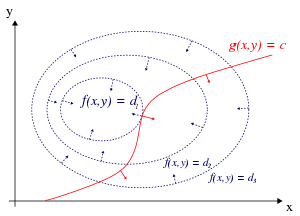
\includegraphics[width=0.50\textwidth]{abstract_img.png}
\end{figure}


\newpage
\tableofcontents
\newpage

\section{Lagrange Multipliers}
%%%%%%%%%%%%%%%%%%%%%%%%%%%%%%%%%%%%%%%%%%%%%%%%%%%%%%%%%%%%%%%%%%%%%%%%%%%%%%%%%%%%%
\subsection{Introduction}

\begin{theorem}(Implicit Function Theorem) \\
    Suppose that $F:\mathbb{R}^{n+1}\to \mathbb{R}$ is $C^{1}$. We will denote points in $\mathbb{R}^{n+1}$ 
    by ($\pmb{x}$,$z$), where $\pmb{x}\in \mathbb{R}^n$ and $z\in \mathbb{R}$. Assume \\
    $$
        F(\pmb{x}_{0},z_{0})=c \hspace{30pt} and \hspace{30pt} \nabla F(\pmb{x}_{0},z_{0})\neq \pmb{0}
    $$
    Then there is a ball $U$ that contains $\pmb{x}_{0}$ and a neighborhood $V$ of $z_{0}$ in $\mathbb{R}$ such that there is a function $z=g(\pmb{x})$ defined for $\pmb{x}$ in $U$ and $z$ in $V$ that satisfies
    $$
        F(\pmb{x},g(\pmb{x}))=c
    $$
    
\end{theorem}

\begin{theorem}(Method of Lagrange Multipliers) \\
    Suppose that $f:U\subset\mathbb{R}^{n}\to \mathbb{R}$ and $g:U\subset\mathbb{R}^{n}\to \mathbb{R}$ are $C^{1}$. Let $\pmb{x}_{0}\in U$ and $g(\pmb{x}_{0})=c$, and let $S$ be the level set for $g$ with value $c$ (i.e these are the set of points $\pmb{x}\in \mathbb{R}^{n}$ that satisfy $g(\pmb{x})=c$).
    Assume $\nabla g(\pmb{x}_{0})\neq \pmb{0}$. \\
    If $f$ achieves a local extremum at $\pmb{x}_{0}$, then there exists $\lambda$ such that
    $$
        \nabla f(\pmb{x}_{0}) = \lambda \nabla g(\pmb{x}_{0})
    $$
\end{theorem}

\begin{proof}
    For the sake of simplicity, take n=3. Then we are dealing with a level surface of the function $g(x,y,x)=c$ though the point $(x_0,y_0,z_0)$.
    By the Implicit Function Theorem we know that there is a function $z=\phi(x,y)$ satisfying $g(x,y,\phi(x,y)) = c$ for $(x,y)$ near $(x_0, y_0)$ and $z$ near $z_0$.
    It follows that locally (near $z_0$), the surface S is the graoh of the function $\phi$. For $\phi$ differentiable and continuous,
    the tangent plane at $(x_0,y_0,z_0)$ to S is given by:
    \begin{equation}
        z = z_0 + \left[\frac{\partial\phi}{\partial x}(x_0,y_0)\right](x-x_0) + \left[\frac{\partial\phi}{\partial y}(x_0,y_0)\right](y-y_0) \tag{1}
    \end{equation}
    We can substitute
    $$
        \frac{\partial\phi}{\partial x} = - \frac{g_x}{g_z} \hspace{30pt}  \hspace{30pt} \frac{\partial\phi}{\partial y} = - \frac{g_y}{g_z}
    $$
    in (1) and obtain:
    $$
        (x-x_0)g_x + (y-y_0)g_y + (z-z_0)g_z = 0
    $$
 
    \begin{equation}
        (x-x_0, y-y_0, z-z_0)\cdot\nabla g(x_0,y_0,z_0) = 0 \tag{2}
    \end{equation}

    At $(x_0,y_0,z_0)$ the tangent planet to the level surface $g$ is orthogonal to $\nabla g(x_0,y_0,z_0)$.
    Now we need to show that every vector tangent to S at $(x_0,y_0,z_0)$ is tangent to every curve in S.
    If $\pmb{v}=(x-x_0,y-y_0,z-z_0)$ is tangent to S, then $\pmb(v)$ is tangent to every path in S given by
    $$
        c(t) = (x_0+t(x-x_0), y_0+t(y-y_0), \phi(x_0+t(x-x_0), y_0+t(y-y_0)))
    $$
    at $t=0$.
    Now, if $(x_0,y_0,z_0)$ is an extremum, then $f(c(t))$ is an extremum when $t=0$ and $c'(0)$ is a tangent vector to S at $(x_0,y_0,z_0)$
    $$
        \left.\frac{d}{dt}f(c(t))\right\vert_{t=0} = \nabla f(x_0)\cdot c'(0) = 0
    $$
    Thus, $\nabla f(x_0)$ is orthogonal to every tangent vector to S at $(x_0,y_0,z_0)$. Since the space orthogonal to this tangent space is a line,
    $\nabla f(x_0,y_0,z_0)$ and $\nabla g(x_0,y_0,z_0)$ are parallel and $\nabla f(x_0,y_0,z_0)$ is a multiple of $\nabla g(x_0,y_0,z_0)$
    $$
        \nabla f(x_0,y_0,z_0) = \lambda \nabla g(x_0,y_0,z_0)
    $$
    The multiple $\lambda$ is called a Lagrange Multiplier.
\end{proof}

\subsection{Single Constraint}
%%%%%%%%%%%%%%%%%%%%%%%%%%%%%%%%%%%%%%%%%%%%%%%%%%%%%%%%%%%%%%%%%%%%%%%%%%%%%%%%%%%%%
\begin{example}
    Find the points closest to the origin on $xy + 3x +z^2 = 9$
\end{example}
The distance from any point $(x,y,z)$ to the origin can be expressed as $\sqrt{x^2+y^2+z^2}$.
We want to minimize this distance subject to the constraint $xy+3x+z^2=9$. We will denote the function we want to minimize as $f$.
We will use the square of the distance formula as it does not change the result but makes the calculations simpler.
We have
$$
    f(x,y,z)=x^2+y^2+z^2 \hspace{30pt}  \hspace{30pt} g(x,y,z)=xy+3x+z^2-9
$$
The Method of Lagrange Multipliers tells us that at the critical points of a function
\begin{equation}
    \nabla f(x,y,z) = \lambda \nabla g(x,y,z)
\end{equation}
We find the gradient of $f$ and $g$
$$
    \nabla f(x,y,x) = <2x,2y,2z>
    \nabla g(x,y,x) = <y+3,x,2z>
$$
After substituting in (1), we get a system of three equations and three variables. For the fourth equation we use the constraint.

\begin{equation*}
    \left\{
    \begin{alignedat}{3}
    % R & L   &  R & L   &  R & L 
        2x= &\lambda(y+3) \\
        2y= &\lambda x \\
        2z= &\lambda 2z \\
        xy +& 3x +z^2 = 9
    \end{alignedat}
    \right.
\end{equation*}

From the third equation we see that $\lambda=1$ and substituting in the first and second we get $x=2$ and $y=1$. Finally, substituting in the last
equation gives us $z = \pm 1$. So, the two critical points are $A=(2,1,1)$ and $B=(2,1,-1)$ and the distance to the origin is $\sqrt{6}$.
We know that at this points on $f$ we will be closest to the origin because any other point we choose on $f$ will give us a bigger distance.

\begin{figure}[h]
    \centering
    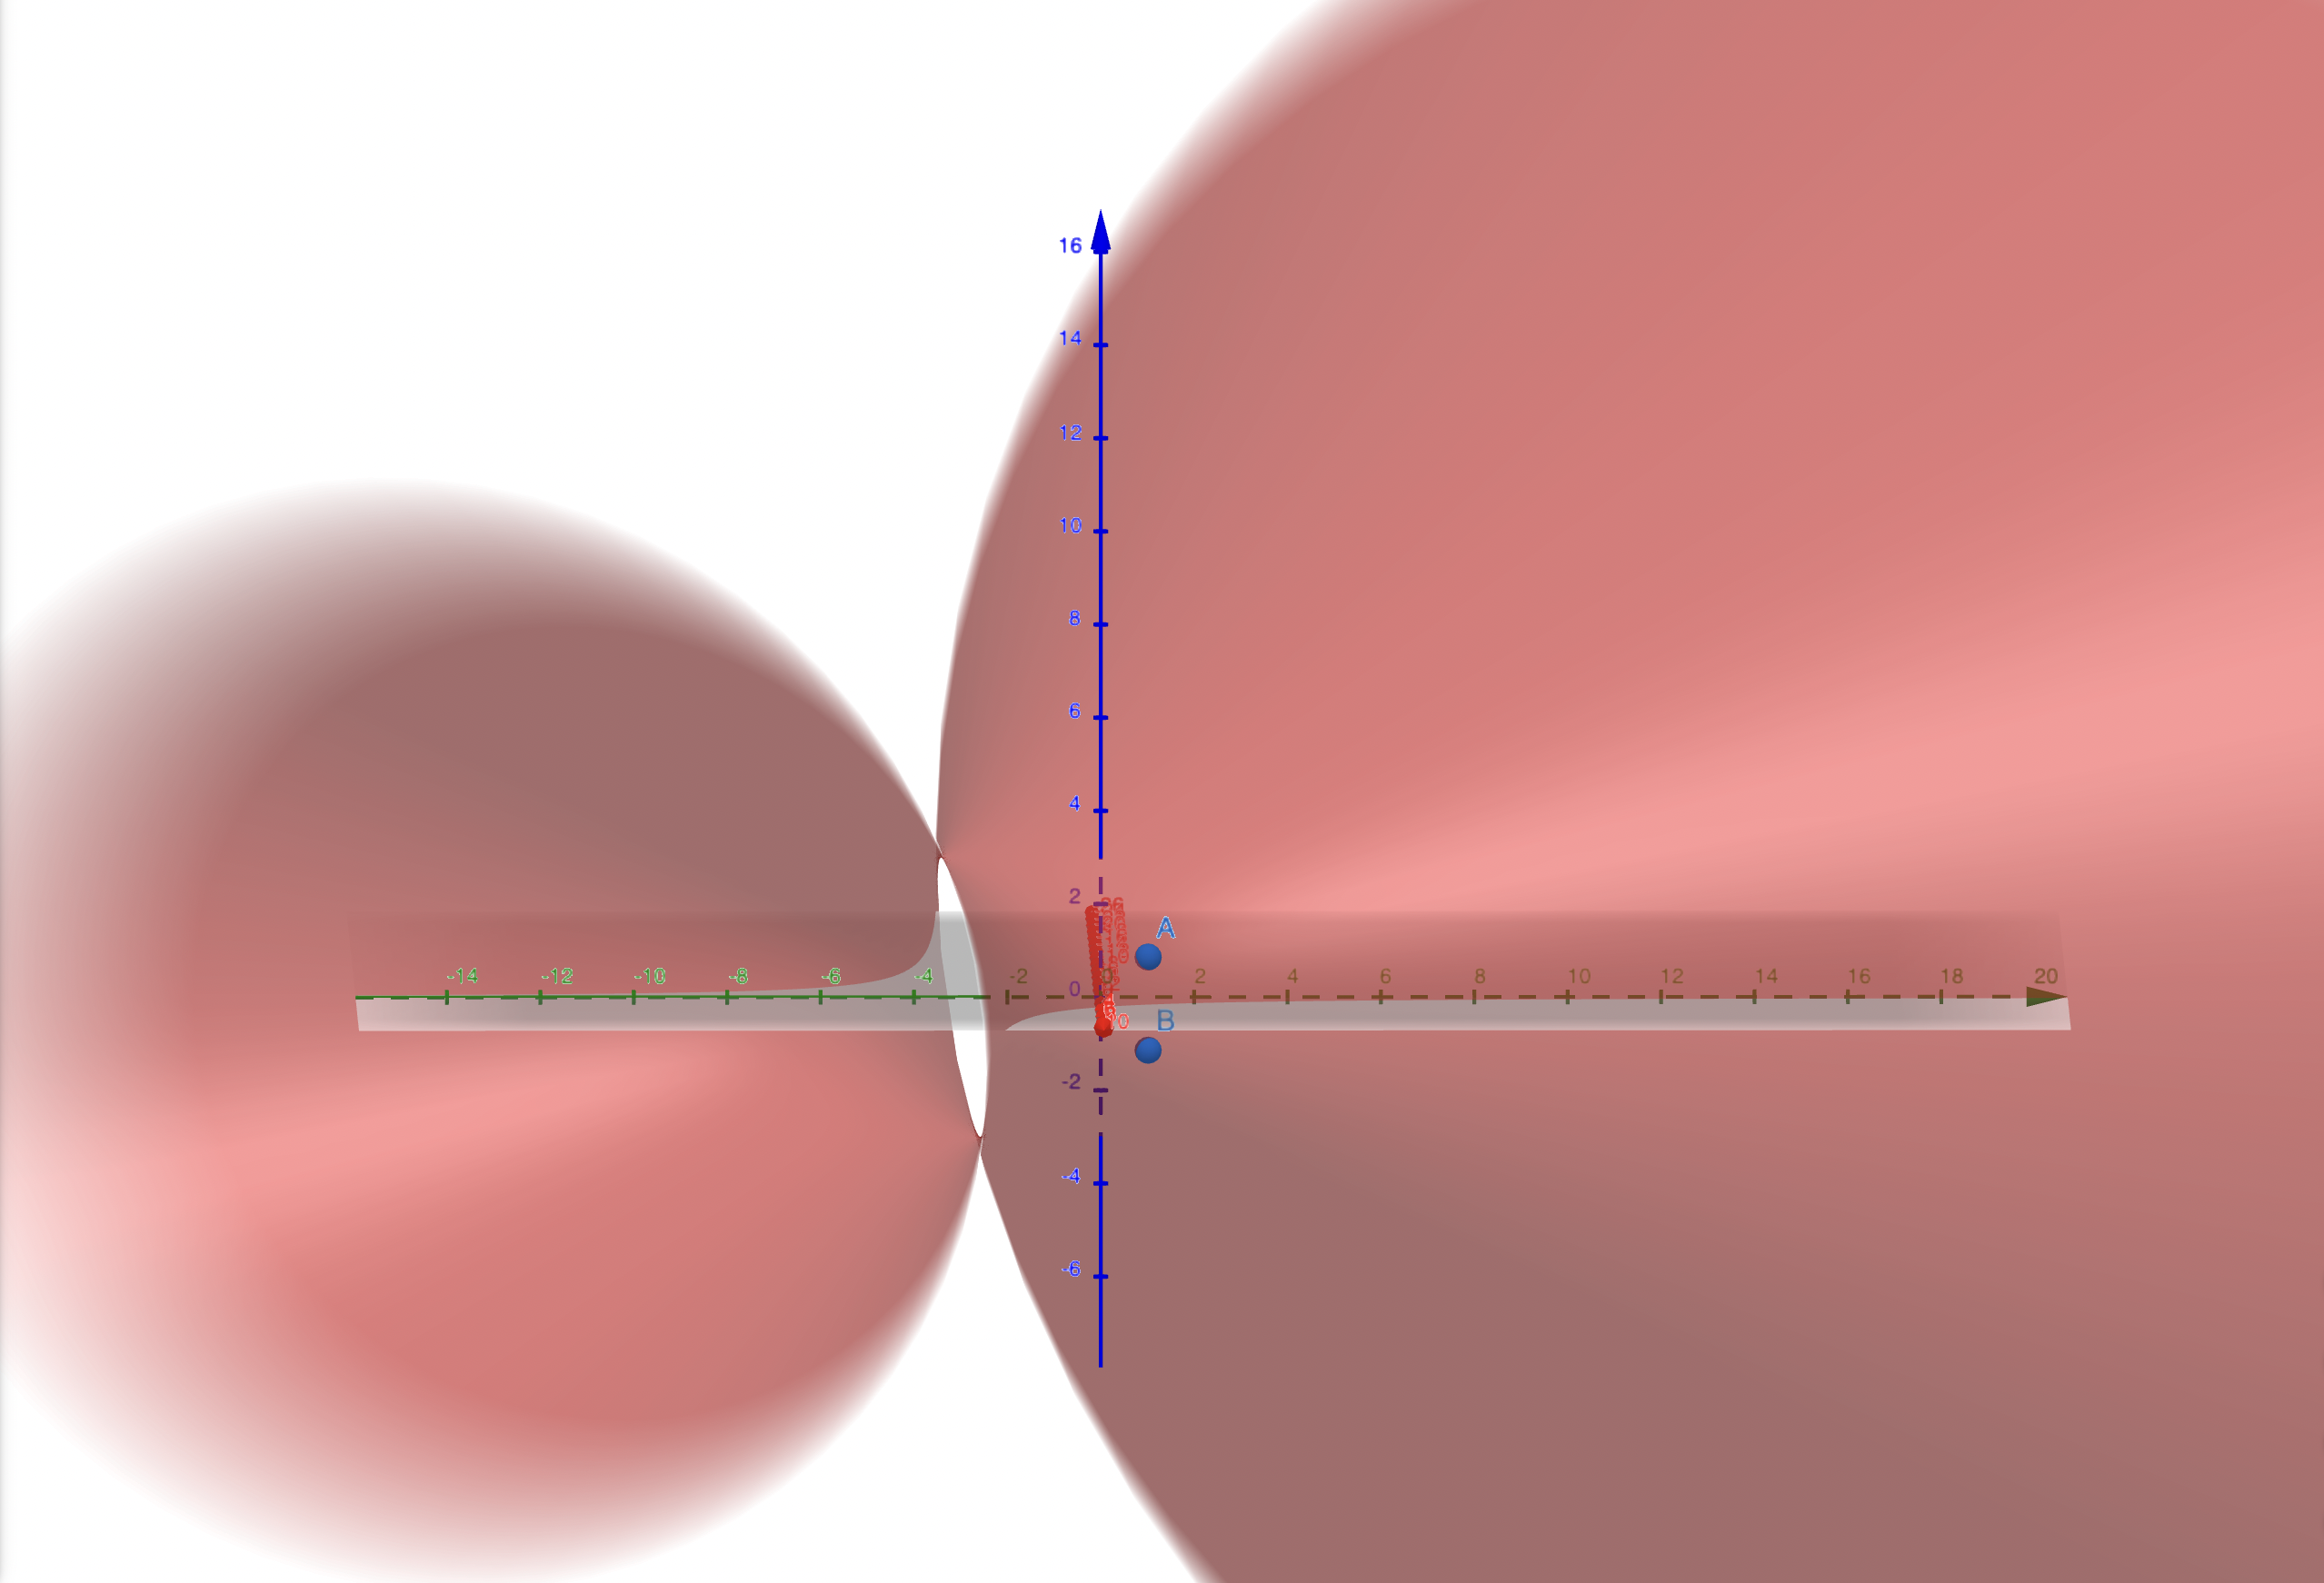
\includegraphics[width=0.9\textwidth]{example1.png}
\end{figure}

\begin{example}
    Find the ellipse $\frac{x^2}{a^2} + \frac{y^2}{b^2} = 1$ that passes through $(3,1)$ and has the smallest area.
\end{example}

The function we are striving to minimize is the area of an ellipse function $A=\pi ab$ that is subject to the constraint
$\frac{9}{a^2} + \frac{1}{b^2} = 1$. We need $a,b>0$. We will denote the function we want to minimize $f(a,b)=\pi ab$
and the constraint $g(a,b)=\frac{9}{a^2} + \frac{1}{b^2}-1$. For $f$ and $g$ $C^1$, for the critical points the method of Lagrange Multipliers gives us
$$    
    \nabla f(x,y,z) = \lambda \nabla g(x,y,z)
$$
$$
    <\pi a, \pi b> = \lambda <-18a^{-3}, -2b^{-3}>
$$
\begin{equation*}
    \left\{
    \begin{alignedat}{3}
    % R & L   &  R & L   &  R & L 
        \pi b= &\lambda(-18)a^{-3} \\
        \pi a= &\lambda (-2)b^{-3} \\
        \frac{9}{a^2} +& \frac{1}{b^2} = 1
    \end{alignedat}
    \right.
\end{equation*}
Solving for $\lambda$ in the first equation and substituting in the second we get

\begin{equation*}
    \left\{
    \begin{alignedat}{3}
    % R & L   &  R & L   &  R & L 
        \lambda= &\frac{\pi ba^{3}}{-18} \\
        a= & \frac{a^3}{9b^2} \\
        \frac{9}{a^2} +& \frac{1}{b^2} = 1
    \end{alignedat}
    \right.
\end{equation*}

Solving the second equation gives us $a=0$ and $9b^2-a^2=0$. $a=0$ is not in out domain. Solving for $b$ gives us $b=\pm \frac{a}{3}$.
Now, we solve the third equation for $a$ and obtain $a=\pm 3\sqrt{2}$.\\
For $a=\pm 3\sqrt{2}$ and $b=\pm \frac{a}{3}$ we get the following choices of $(a,b)$: $(3\sqrt{2}, \sqrt{2}),\\
(3\sqrt{2}, -\sqrt{2}), (-3\sqrt{2}, \sqrt{2}), (-3\sqrt{2}, -\sqrt{2})$.
Since we are interested in $a,b>0$ the only choice is $(3\sqrt{2}, \sqrt{2})$. 

\begin{figure}[h]
    \centering
    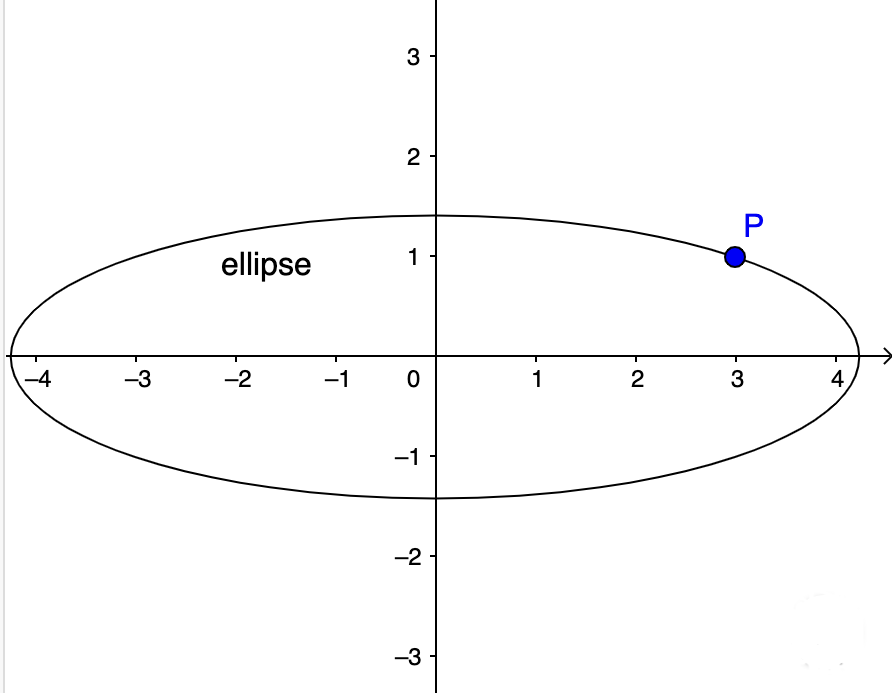
\includegraphics[width=0.50\textwidth]{example2.png}
\end{figure}



\subsection{Multiple Constraints}
%%%%%%%%%%%%%%%%%%%%%%%%%%%%%%%%%%%%%%%%%%%%%%%%%%%%%%%%%%%%%%%%%%%%%%%%%%%%%%%%%%%%%

\subsection{Second Derivative Test}
%%%%%%%%%%%%%%%%%%%%%%%%%%%%%%%%%%%%%%%%%%%%%%%%%%%%%%%%%%%%%%%%%%%%%%%%%%%%%%%%%%%%%

\subsection{Lagrangian}
%%%%%%%%%%%%%%%%%%%%%%%%%%%%%%%%%%%%%%%%%%%%%%%%%%%%%%%%%%%%%%%%%%%%%%%%%%%%%%%%%%%%%

\section{Applications}
%%%%%%%%%%%%%%%%%%%%%%%%%%%%%%%%%%%%%%%%%%%%%%%%%%%%%%%%%%%%%%%%%%%%%%%%%%%%%%%%%%%%%

\end{document}
